\section{How to Get Started}
\medskip 
To get started, TalkBox configuration is composed of two modes allowing you to configure and playback the TalkBox device. You can toggle between these two modes by clicking the "Switch Modes" button in the corner of the bottom left panel of the configuration app. The mode selection that the configuration app is currently in will be displayed in text above the "Switch Modes". 

\medskip

1. Playback Mode

\medskip
\newline
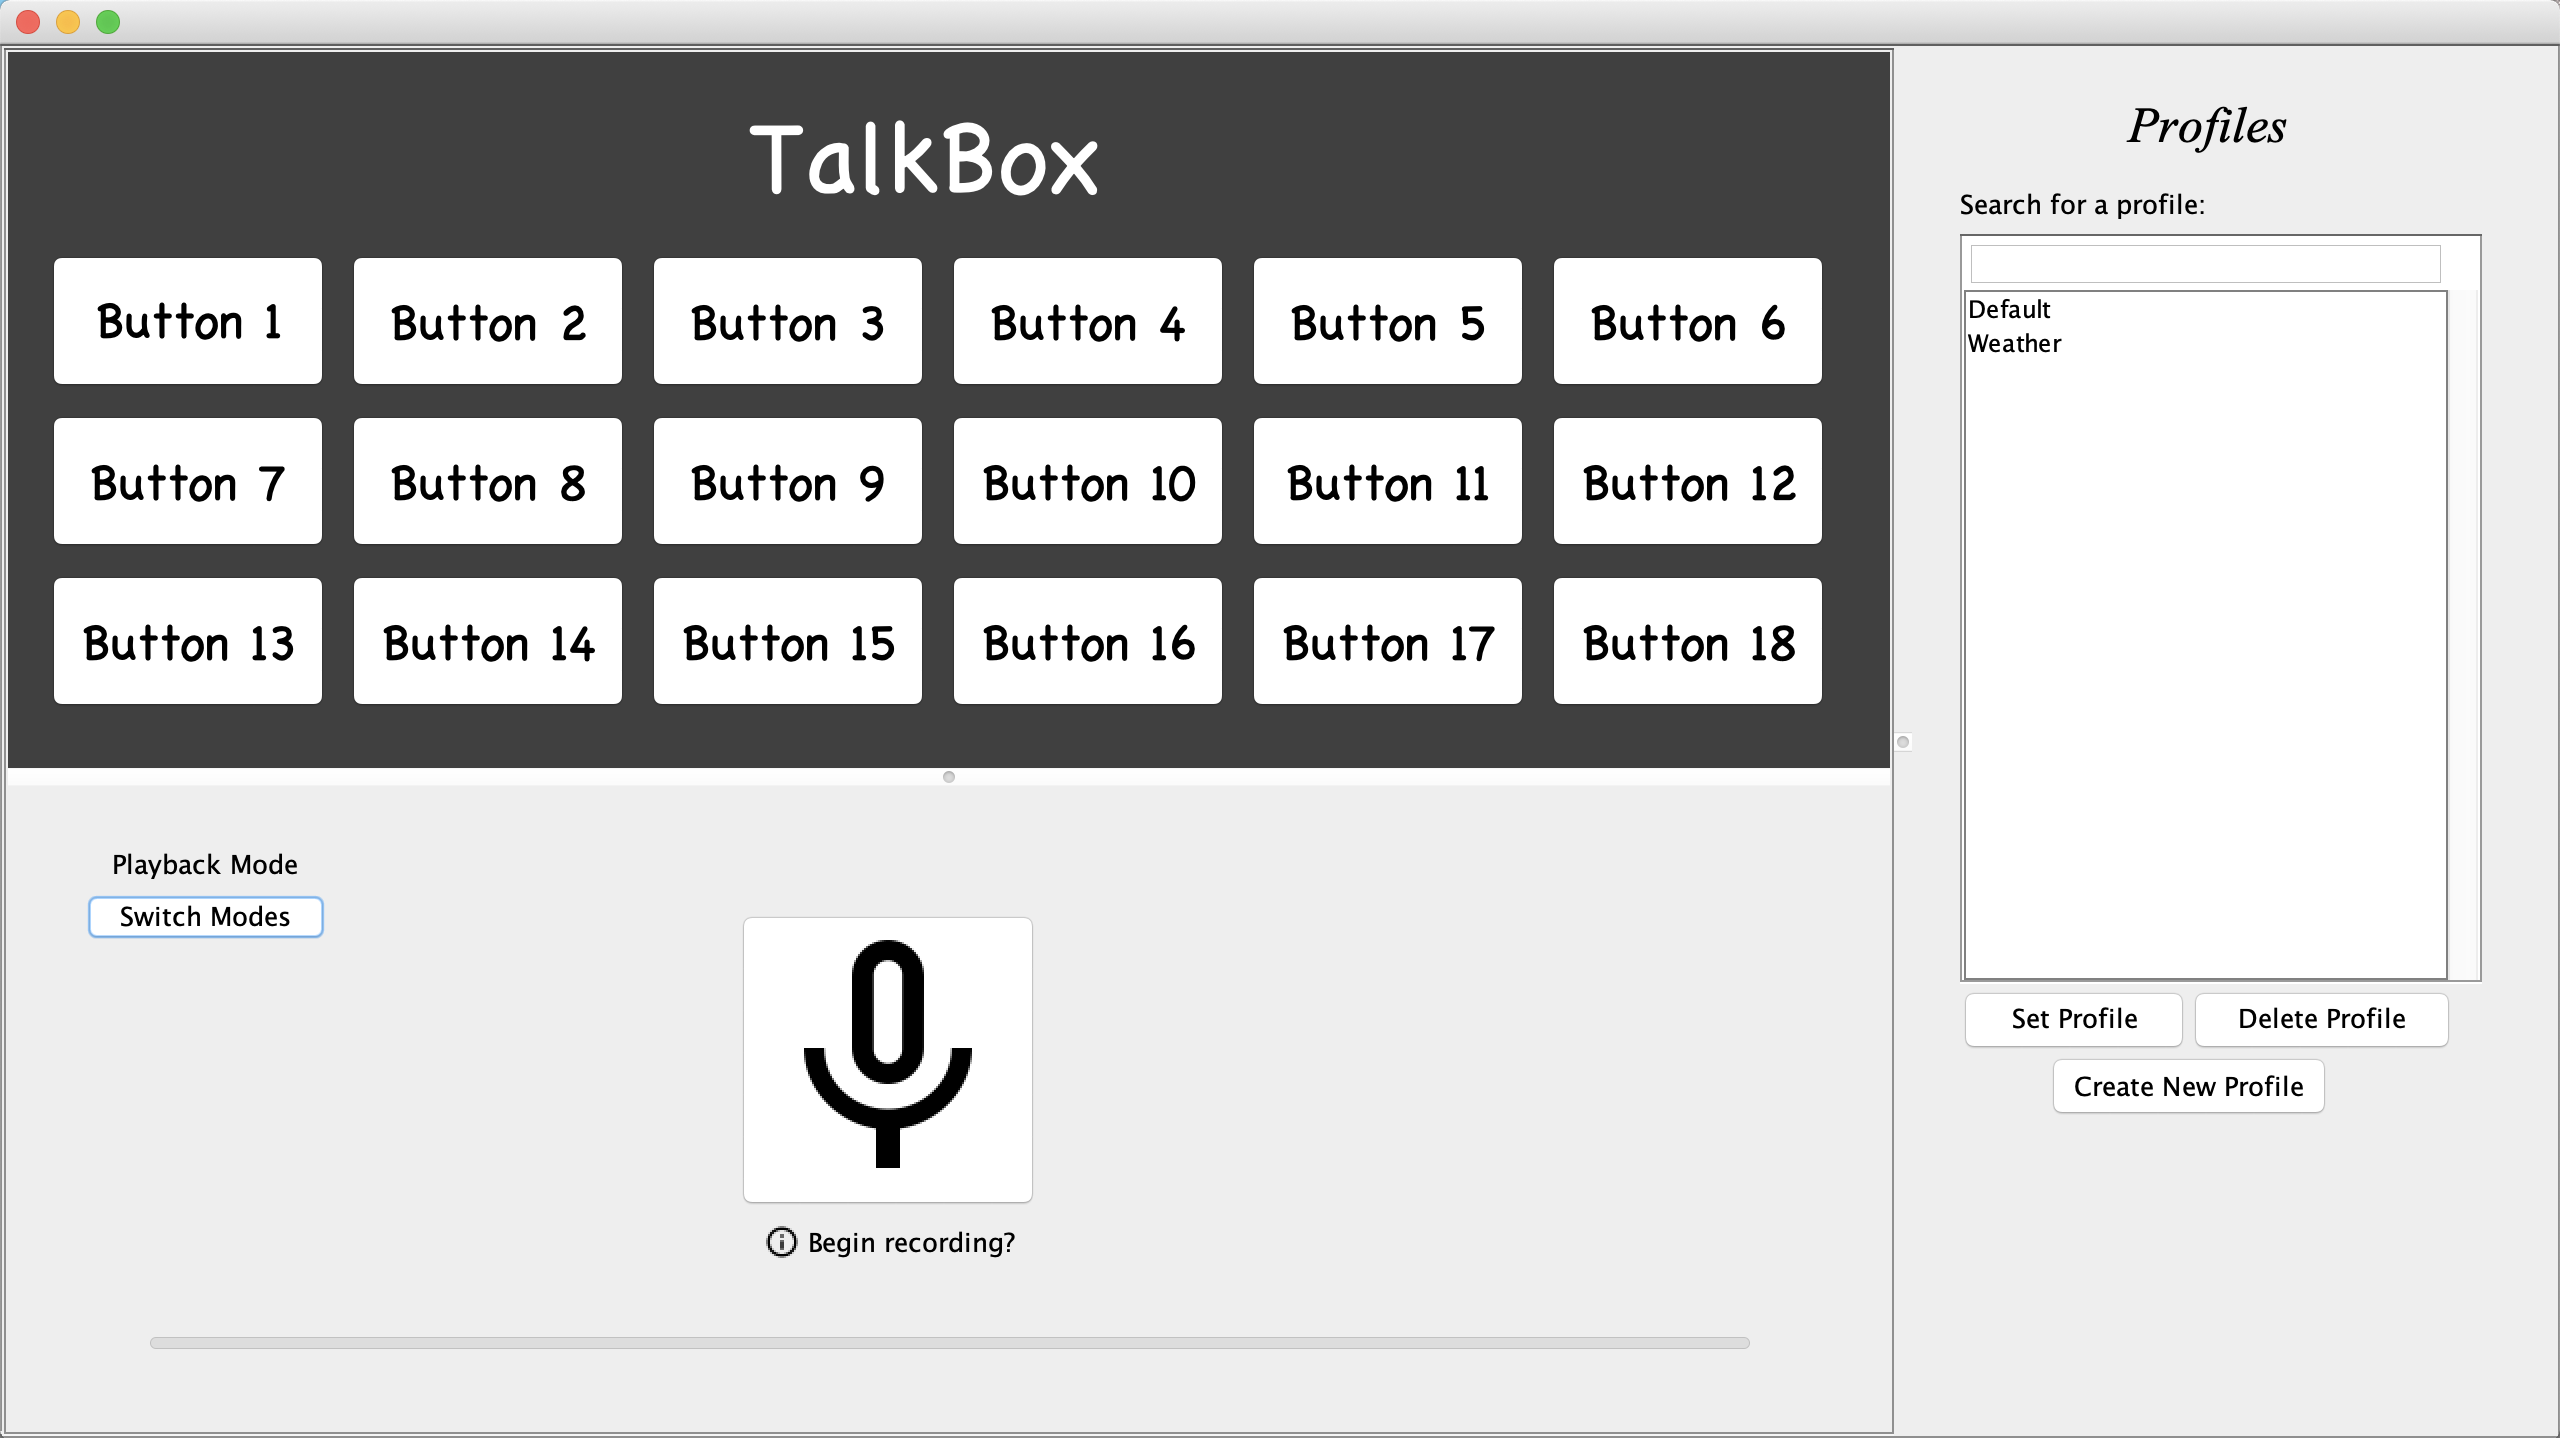
\includegraphics[width=\textwidth]{playback.png}
\medskip

In playback mode, the TalkBox device is simulated in the upper left panel. By clicking on the buttons, you can play back the recordings as the settings that the TalkBox device is currently set to. 
\medskip
\newpage

2. Edit Mode

\medskip

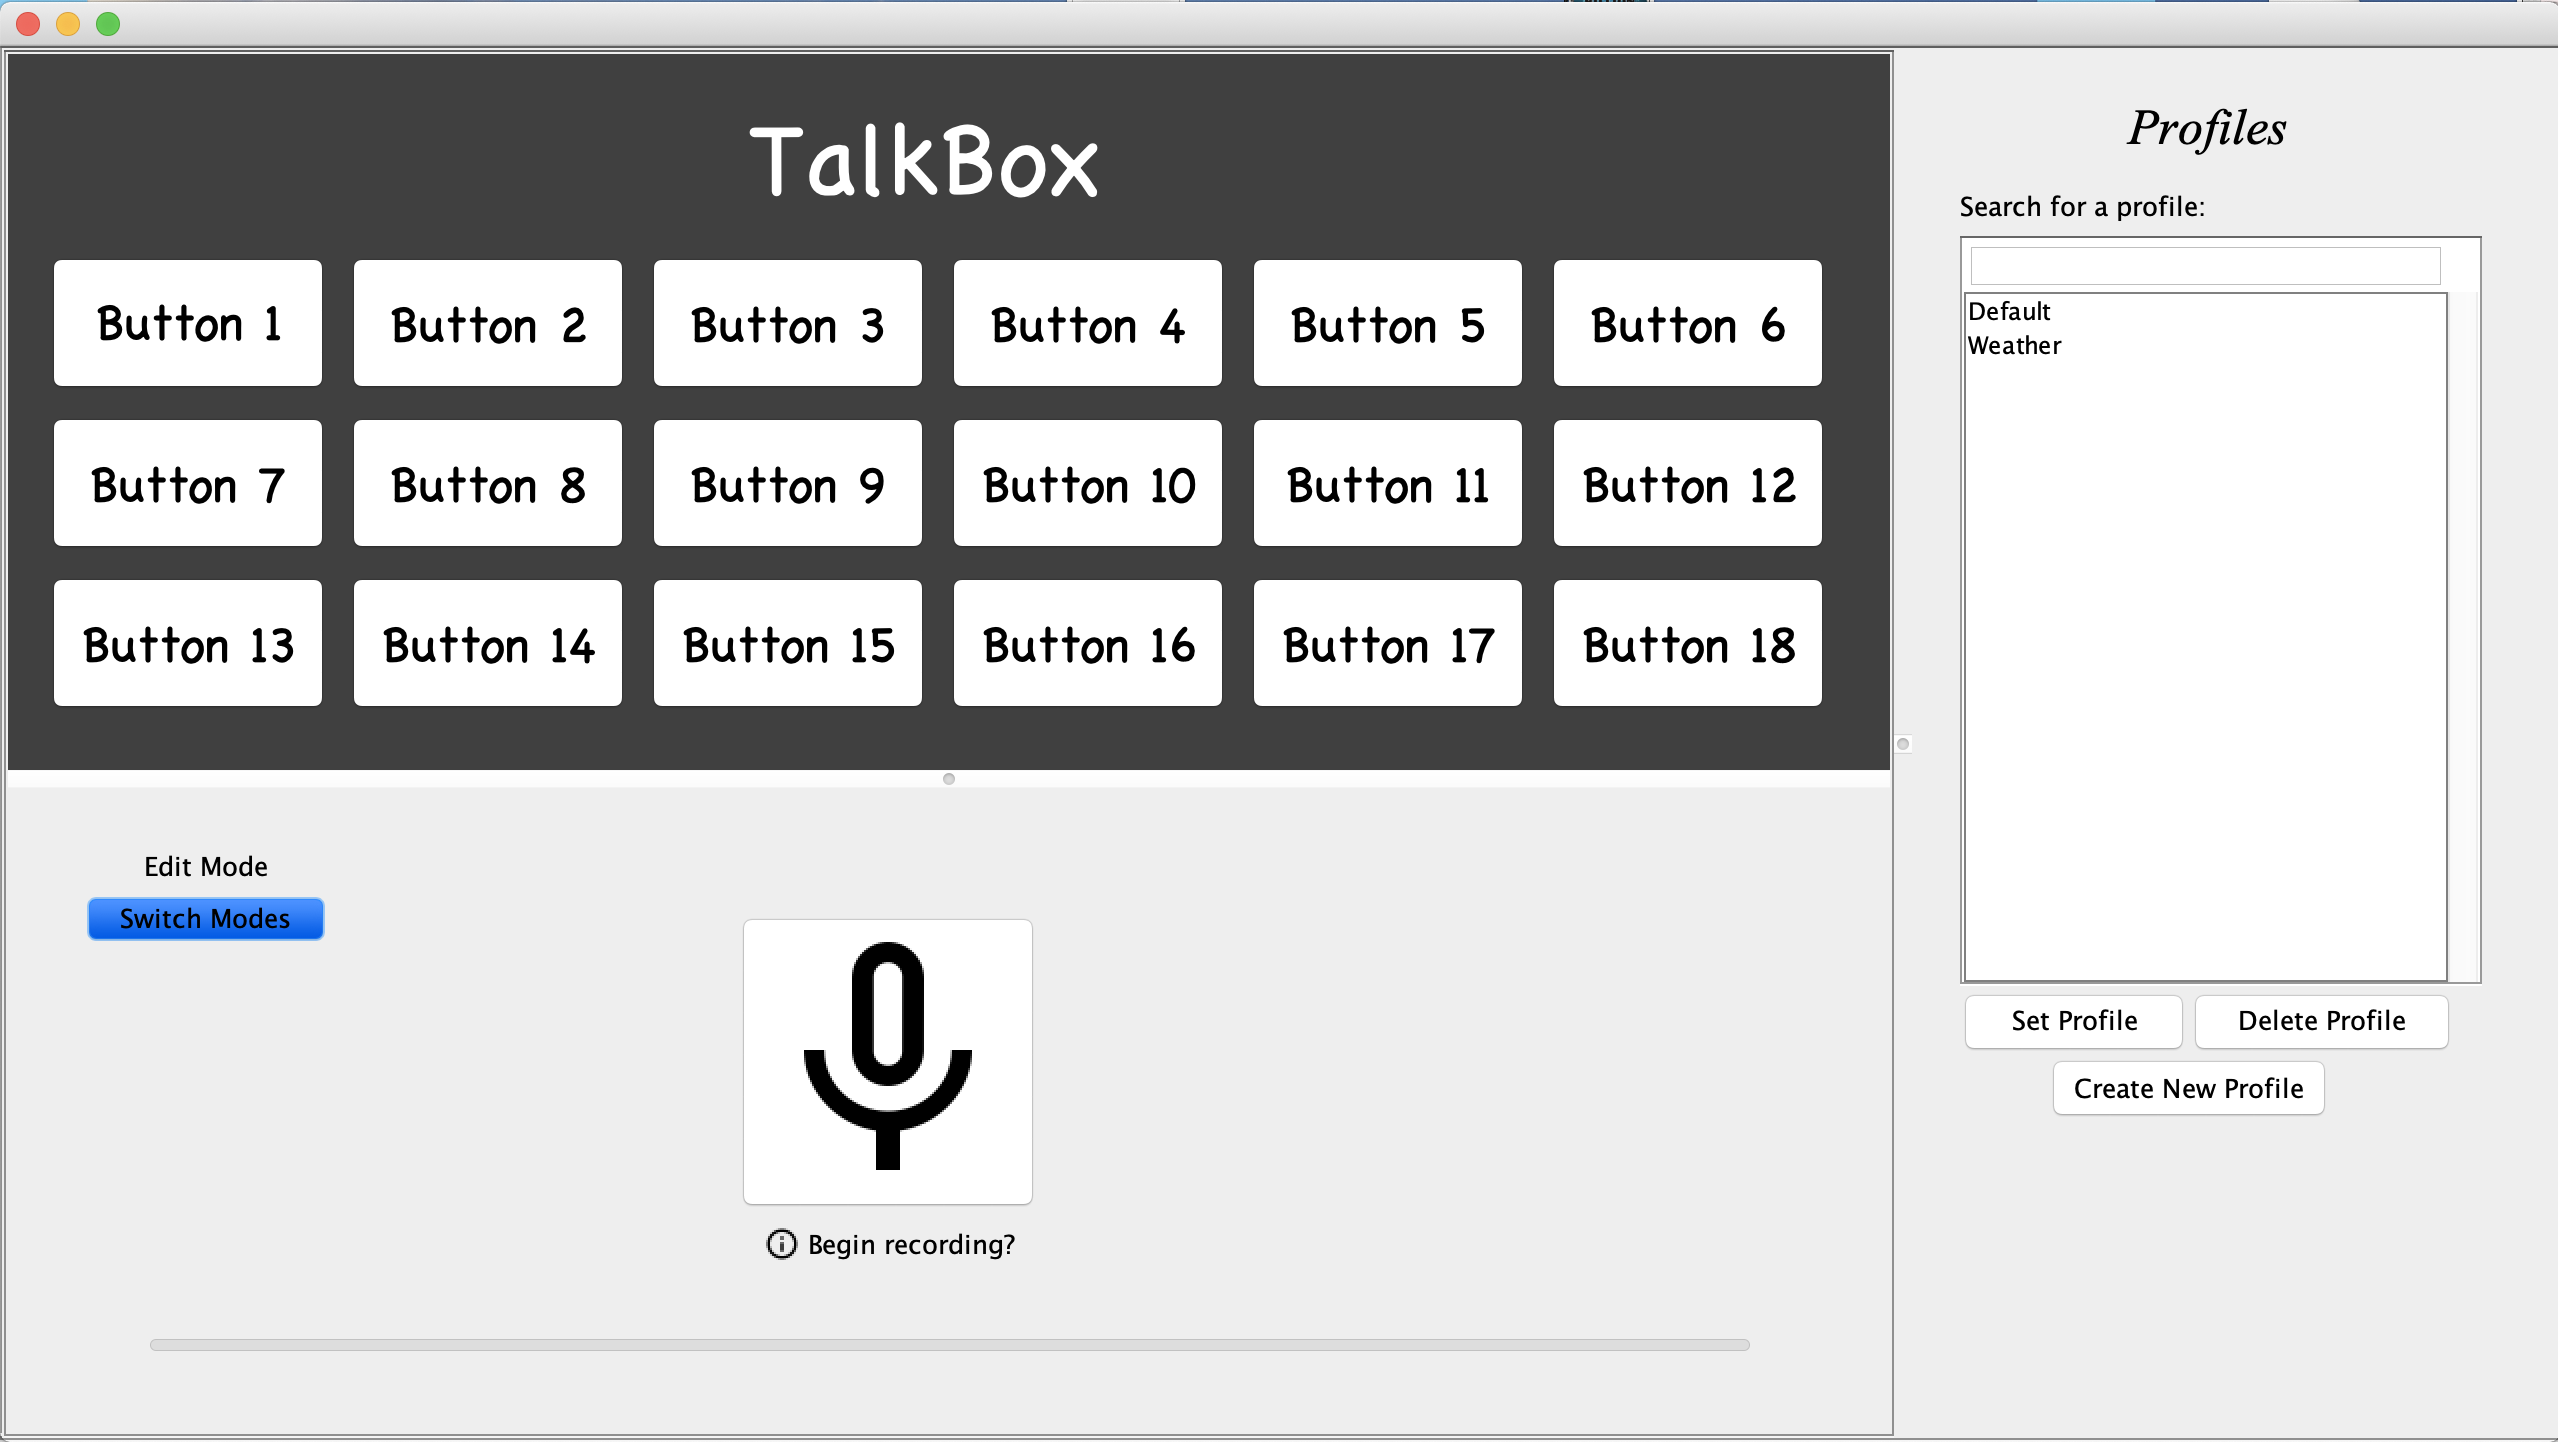
\includegraphics[width=\textwidth]{editmode.png}
\medskip

In edit mode, you can set up the configuration of the TalkBox device. In the profiles panel (on the right of the configuration app, you can load previously saved audio profiles, or create a new profile. When a profile is selected, its set of audio buttons are displayed in the simulation panel (top left of the configuration app). You can play back the audio files associated with buttons by clicking the buttons in the simulator. 

\newline
\medskip
To edit a specific button, click on the button you wish to edit. You can then click the "Record" button to record an new audio file, or select a previously saved audio file. To change the label of the button, select the button and input the new label name in the text box beside "Button Label:". The new label will now appear on the TalkBox simulator on the selected button. 






